\chapter{INTRODUÇÃO}
\label{chap:introduction}

Citar um acronimo: \ac{DoF}, \ac{FRVF}.

\lipsum[1-2]

\chapter{OBJETIVO}
\label{chap:objetive}

Citação na linha \citeonline{earnshaw2014virtual}.
Citação singular: \cite{earnshaw2014virtual}. Citação múltipla: \cite{azuma1997survey, earnshaw2014virtual}.

\section{Tema a}

\lipsum[1]

\section{Tema b}

\lipsum[1]

\chapter{PROCEDIMENTO EXPERIMENTAL} 
\label{chap:methodology}

Deve conter a descrição da área de estudo e dos materiais (banco de dados, coleta de dados, imagens, etc) e dos procedimentos metodológicos (experimentos, entrevistas, métodos estatísticos, etc) que serão empregados na realização do trabalho, de maneira que outros pesquisadores possam reproduzir o estudo. Pode ser apresentada na forma de subdivisões abaixo.

\begin{itemize}
	\item \large \textbf{AHA}: \large \textit{The American Heart Association Database for Evaluation of Ventricular Arrhythmia Detectors}- formada por 80 registros de 35 minutos cada.
	\item \large \textbf{MIT–BIH}: \large \textit{The Massachusetts Institute of Technology–Beth Israel Hospital Arrhythmia Database} - formada por 48 registros de 30 minutos cada.
	\item \large \textbf{ESC}: \large \textit{The European Society of Cardiology ST-T Database} (90 records of 2 hours each) - formada por 90 registros de 2 horas cada.
	\item \large \textbf{NST}: \large \textit{The Noise Stress Test Database} - formada por 12 registros de 30 minutos e 3 registros de apenas ruído.
	\item \large \textbf{CU}: \large \textit{The Creighton University Sustained Ventricular Arrhythmia Database} - formada por 35 registros de 8 minutos cada.
\end{itemize}

\section{MIT-BIH}

\begin{figure}[htb]
	\begin{center}  
		\includegraphics[scale=0.6]{images/haptic.png}
	\end{center}
	\caption{Exemplos de batimento. }
	\legend{Fonte: \cite[p. 13]{yew2017immersive}}
	\label{fig_mitbih}
\end{figure}

\subsection{Sub seção}

\begin{table}[htb]
	\centering
	\caption{Registros utilizados e número de representantes de cada classe para cada uma das partições. }
	\begin{adjustbox}{width=1\textwidth}
		\label{tabela-particoes}
		\begin{tabular}{|c|c|c|c|c|c|c|}
			\hline
			\rowcolor[HTML]{D0D0D0}
			Partições                     & Registros                                                                                                                                              & Classe N & Classe SVEB & Classe VEB \\ \hline
			\hline      
			\cellcolor[HTML]{EFEFEF}DS1   & 101, 106, 108, 109, 112, 114, 115, 116, 118, 119, 122, 124, 201, 203, 205, 207, 208, 209, 215, 220, 223, 230 & 45543    & 782         & 3469       \\ \hline        
			\cellcolor[HTML]{EFEFEF}DS11  & 101, 106, 108, 109, 114, 115, 116, 119, 122, 209, 223                                                                                                  & 22249    & 474         & 1615       \\ \hline      
			\cellcolor[HTML]{EFEFEF}DS12  & 112, 118, 124, 201, 203, 205, 207, 208, 215, 220, 230                                                                                                  & 23294    & 308         & 1854       \\ \hline  
			\cellcolor[HTML]{EFEFEF}DS2   & 100, 103, 105, 11, 113, 117, 121, 123, 200, 202, 210, 212, 213, 214, 219, 221, 222, 228, 231, 232, 233, 234  & 44049    & 1808        & 3143       \\ \hline
			\rowcolor[HTML]{B8B8B8} 
			\cellcolor[HTML]{EFEFEF}Total &                                                                                                                                                        & 89592    & 2590        & 6612       \\ \hline
		\end{tabular}
	\end{adjustbox}
\end{table}

\subsubsection{Sub sub seção}

Exemplo de equação a seguir:

\begin{equation}
w_{ij} = e_{i,j} = \sqrt{(x_i - x_j)^2 + (y_i - y_j)^2 + (z_i - z_j)^2},
\label{eq:edge}
\end{equation}

\begin{algorithm}
	\caption{PSO com fator de inércia}
	\label{pseudoPSO}
	\begin{algorithmic}[1]
		\State Inicia a população de partículas com velocidades e posições aleatórias
		\While{Condições de parada não são atingidas}
		\For{Cada partícula $i$}
		\State Atualiza a velocidade da partícula de acordo com \ref{eq:1}
		\State Atualiza a posição da partícula usando \ref{eq:2}
		\State Avalia o $fitness$  {$f({X}_i)$}
		\If{$f({X}_i)>f({Pbest}_i)$}
		\State ${Pbest}_i \gets {X}_i$
		\EndIf
		\If{$f({X}_i)<f({Gbest})$}
		\State ${Gbest} \gets {X}_i$
		\EndIf
		\EndFor
		\EndWhile
	\end{algorithmic}
\end{algorithm}

\begin{equation}
\label{eq:sigmoide}
s(v)=\frac{1}{1+\exp(-v)}
\end{equation}

\begin{figure}[htb]
	\begin{center}  
		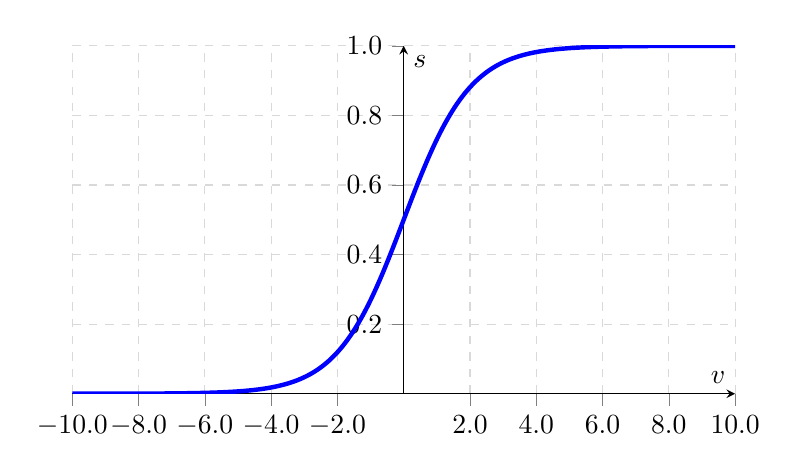
\begin{tikzpicture}
		\begin{axis}[
		legend pos=north west,
		axis x line=middle,
		axis y line=middle,
		x tick label style={/pgf/number format/fixed,
			/pgf/number format/fixed zerofill,
			/pgf/number format/precision=1},
		y tick label style={/pgf/number format/fixed,
			/pgf/number format/fixed zerofill,
			/pgf/number format/precision=1},
		grid = major,
		width=10cm,
		height=6cm,
		grid style={dashed, gray!30},
		xmin=-10,     % start the diagram at this x-coordinate
		xmax= 10,    % end   the diagram at this x-coordinate
		ymin= 0,     % start the diagram at this y-coordinate
		ymax= 1,   % end   the diagram at this y-coordinate
		%axis background/.style={fill=white},
		xlabel=$v$,
		ylabel=$s$,
		tick align=outside,
		enlargelimits=false]
		% plot the stirling-formulae
		\addplot[domain=-10:10, blue, ultra thick,samples=500] {1/(1+exp(-x))};
		\end{axis}
		\end{tikzpicture}
	\end{center}
	\caption{Comportamento da função sigmóide para valores entre -10 e 10.}
	\label{fig_sigmoide}
\end{figure}

\chapter{RESULTADOS}

\lipsum[1-2]

\chapter{DISCUSSÃO}

Apresentar as discussões dos resultados obtidos no presente estudo com aqueles de publicações anteriores, destacando qual foi a sua contribuição sobre a temática abordada.

\chapter{CONCLUSÃO}

Mencionar as principais conclusões da dissertação destacando os pontos mencionados nos objetivos específicos.

\chapter{RECOMENDAÇÕES}

Mencionar os possíveis desdobramentos da pesquisa e as sugestões para a continuação do trabalho.
